\documentclass[emulatestandardclasses]{scrartcl}
\usepackage{graphicx}
\usepackage{color}
\usepackage[ngerman]{babel}
\usepackage{hyperref}
\usepackage[utf8]{inputenc}
\usepackage{fullpage}
\usepackage{calc} 
\usepackage{enumitem}
\usepackage{titlesec}
\newcommand{\todo}[1]{\textcolor{red}{TODO: #1}\PackageWarning{TODO:}{#1!}}
\date{\vspace{-3ex}}
\begin{document}

\title{
	\includegraphics*[width=0.75\textwidth]{ErstesSem/images/hu_logo.png}\\
	\vspace{24pt}
	Hegels System}
\subtitle{Proseminar WS 17/18\\
          Prof. Dr. Andreas Arndt\\
          Theologische Fakult"at \\ 
          Humboldt Universit"at zu Berlin}
\author{Lennard Wolf\\
        \small{\href{mailto:lennard.wolf@student.hu-berlin.de}{lennard.wolf@student.hu-berlin.de}}}
\maketitle
\begin{abstract}
Hegels System liegt nicht in einem fertigen Zustand vor, sondern nur als \emph{work in progress}, in Grundrissen bzw. Grundlinien und Ausarbeitungen einzelner Teile, zum Teil - wie in den Vorlesungen - in immer neuen Anläufen. Entsprechend geht es weniger darum, die einzelnen Teile des Hegelschen Systementwurfs (Logik, Naturphilosophie, Geistesphilosophie) im Einzelnen zu referieren, als vielmehr um die Frage, wie sich diese Teile zueinander verhalten und was ihr Gravitationszentrum ist.

\end{abstract}
\newpage

\tableofcontents
\listoffigures
\newpage


\section{Einf"uhrungssitzung\\(17.10.17)}

\subsection{Organisatorisches}

\begin{itemize}
  \item Moodle-PW: 
\end{itemize}

\subsubsection{Literatur}

\begin{itemize}
  \item G.F.W. Hegel: Enzyklopädie der philosophischen Wissenschaften im Grundrisse. Philosophische Bibliothek Bd.33, Meiner Verlag 1830.
  \item Walter Jaeschke: Hegel-Handbuch. Leben – Werk – Schule, 3.Auflage 2016.     
  \item Walter Jaeschke und Andreas Arndt: Die Klassische Deutsche Philosophie nach Kant. Systeme der reinen Vernunft und ihre Kritik, München 2012 (Kap. über Hegel).     
  \item Pirmin Stekeler-Weithofer: Philosophie des Selbstbewusstseins. Hegels System als Formanalyse von Wissen und Autonomie, Frankfurt/M 2005.
\end{itemize}


\subsection{Einf"uhrung - Worum wird es gehen?}

\subsubsection{Fragen}

\begin{itemize}
  \item Verhältnis Objektiver Geist/Absoluter Geist?
  \item Was ist mit Ende der Philosophie/Weltgeschichte gemeint?
  \item Was macht ein System aus und was ist das Systematische bei Hegel?
\end{itemize}

\subsubsection{Welches "`System"'?}

\begin{itemize}
  \item \emph{Enzyklopädie der philosophischen Wissenschaften}: Kompendium der gelehrten Thesen
  \item System bleibt in Grundrissen/Versuchen $\rightarrow$ Nicht fertig/abgeschlossen!
  \item Verein der Freunde des Verewigten: "`Letztgültige Herausgabe"' von Hegels Schriften (Zusammenarbeit Schüler und Witwe) - Mit Zusätzen, die möglicherweise nicht im Geiste Hegels waren
  \item Grundlinien: Grundrisse der Grundrisse (Rechtsphilosophie: Objektiver Geist)
  \item Doch der Grundriss ist nicht die Ausführung und der Inhalt des Systems
  \item Kant: die Methode - auch bei Hegel.
  \item Lukasz: \emph{Was ist orthodoxer Marxismus?} "`Orthodoxie bezieht sich ausschließlich auf die Methode."'
\end{itemize}

\subsubsection{Grenzen}

\begin{itemize}
  \item Es gibt keine Philosophie des subjektiven Geistes $\rightarrow$ hat sich seit der Enzyklopädie natürlich weiter entwickelt, doch dies wurde nie offiziell schriftlich festgehalten in der Form der Enzyklopädie
  \item Hegel wird Position des "`Absoluten Idealismus"' nachgesagt, doch woher stammt dies?
  \item Suhrkamp Ausgabe wissenschaftlich problematisch $\rightarrow$ Authentizität unklar! 
  \item Prokustes Bett: Empirie findet keinen Platz $\rightarrow$ Marx: "`Hegel interessiert sich nicht für die Logik der Sache, sondern die Sache der Logik."' (1943)
\end{itemize}

\subsection{Materialismus vs. Idealismus}

\begin{itemize}
  \item Welche Freiheit wird thematisiert: Freiheit gegenüber Staat oder gegenüber Natur?
  \item Vorschlag: "`Idealrealismus"'
  \item Hegelscher "`Idealismus"': Selbstgesetzgebung/Autonomie der Vernunft - kann nicht aus der Sinnenwelt geborgt sein!
  \item "`Materialismus"': Konsequenter Realismus
  \item Jede Art von Dualismus bringt Gegensatz von Ding und Erscheinung logischerweise immer mit sich
  \item Hegel: Ding an sich ist ("`nur"') eine Abstraktion; Weiter: wenn das endliche nicht ein letztes ist dann ist jedes ???? idealistisch
  \item Geistige Realität ist doch auch endlich: zB der Staat
  \item Monismus sollte für Hegel das Ziel des Idealismus sein, und so waren die französischen Materialisten zu seiner Zeit für ihn die größten Idealisten
  \item "`Verhältnisse in der Gesamtheit"'
\end{itemize}

\subsection{System und Methode}

\begin{itemize}
  \item Kant: System und Methode gehen zusammen
  \item Wissenschaftlichkeit wird durch Methode gestiftet, und durch die Wissenschaft die Systemform
  \item Hegel: Ein \emph{Ganzes} der Erkenntnis als System soll an die Stelle des bloßen Aggregats von Erkenntnissen kommen: "`Das Wahre ist das Ganze"'.
  \item Ganzes ist mehr als nur ein Aggregat!
  \item "`System der Vernunft"': Unsere Vernunft ist \emph{in sich} systematisch strukturiert. Daher erscheint uns die Natur als systematisch.
  \item "`Die menschliche Vernunft ist ihrer Natur nach architektonisch, d. i. sie	 betrachtet alle Erkenntnisse als gehörig zu einem möglichen System und	 verstattet daher auch nur solche Principien, die eine vorhabende Erkenntniß wenigstens nicht unfähig machen, in irgend einem System mit anderen	zusammen zu stehen."' (Kritik der reinen Vernunft)
  \item Die Vernunfteinheit ist die Einheit des Systems
\end{itemize}


\newpage
\section{"Uber den Professor}
Prof. Dr. Andreas Arndt ist..


%\begin{figure}[h]
%	\centering
%	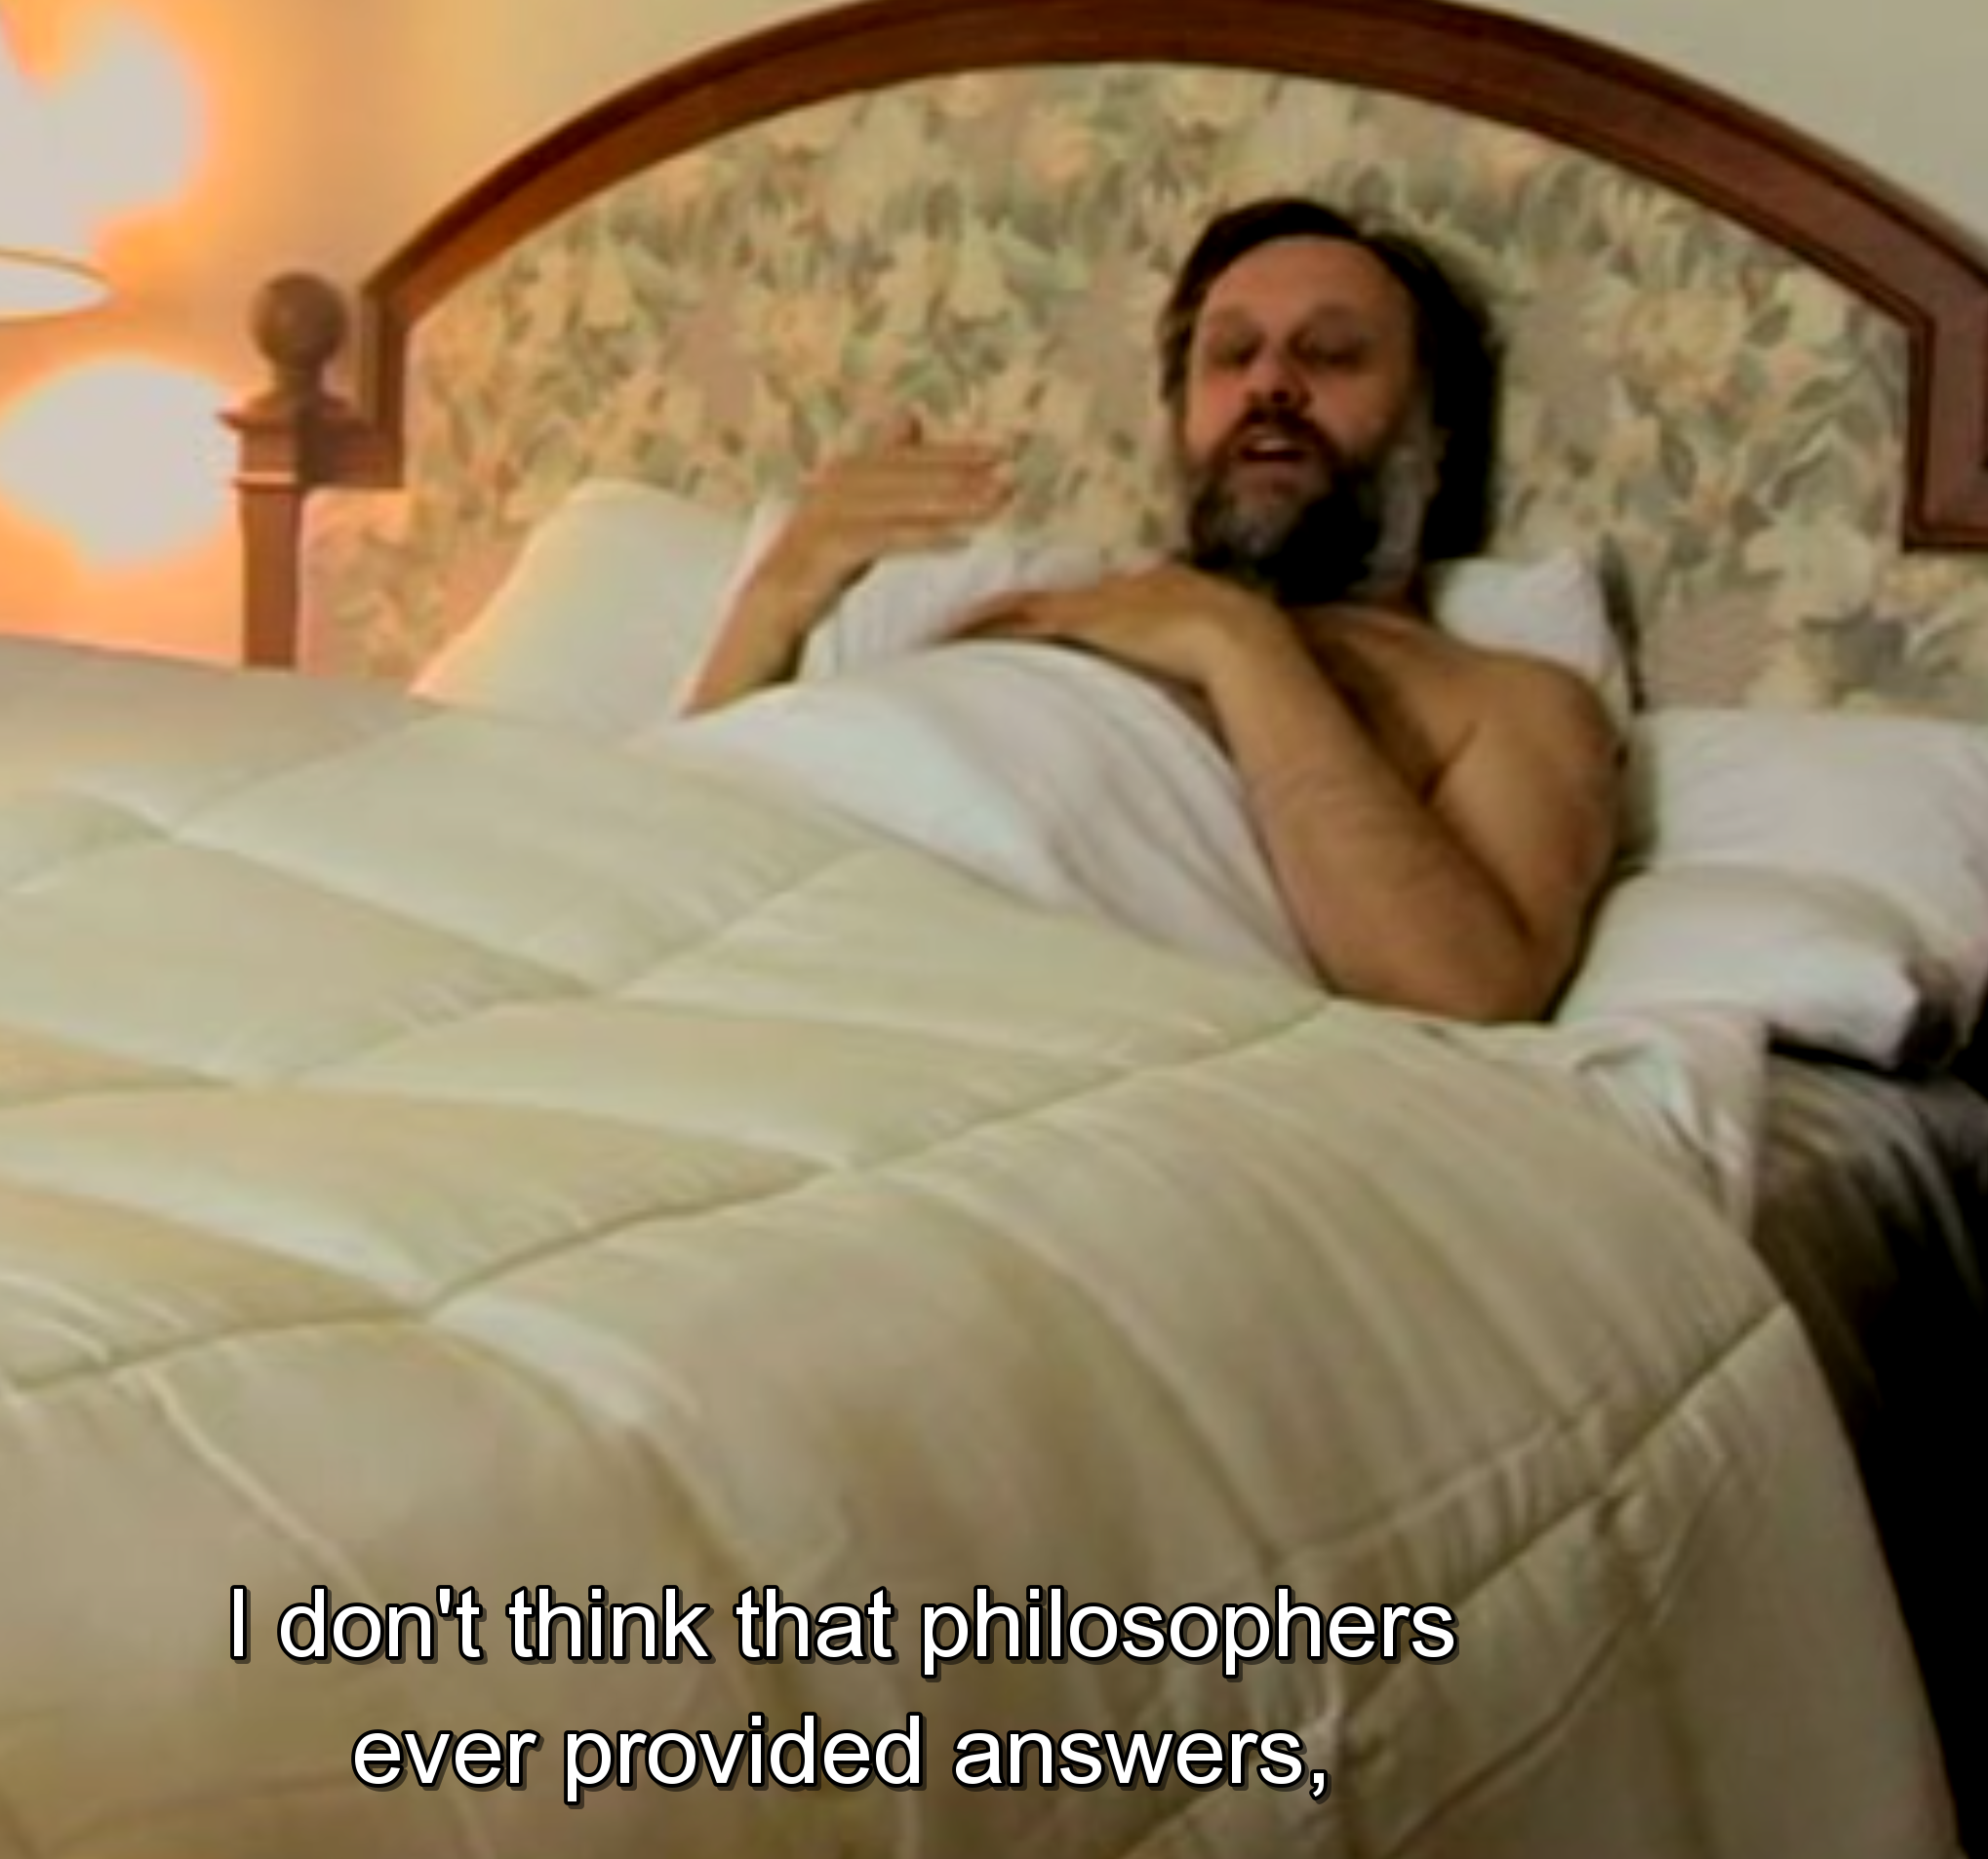
\includegraphics[width=0.5\textwidth]{images/template.png}
%	\caption{Template Bild}
%	\label{fig:template}
%\end{figure}

\end{document}
